\documentclass[margin=8pt]{standalone}
\usepackage{tkz-euclide}
\begin{document}
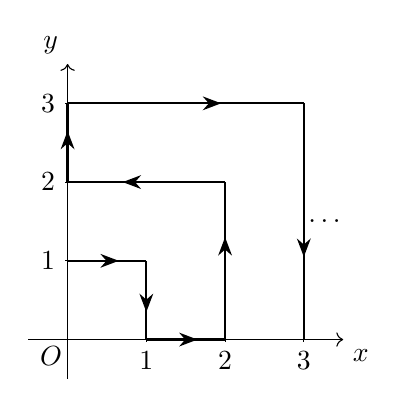
\begin{tikzpicture}[
    decoration={
        markings,% switch on markings
        mark=at position .65 with {\arrow[black]{Stealth}}}
    ]
\usetikzlibrary{shapes.geometric,decorations.markings}
\tkzDefPoints{0/0/O}
%\tkzDefPoints{0/1/A_{1},1/1/A_{2},1/0/A_{3},2/0/A_{4},2/2/A_{5},0/2/A_{6},0/3/A_{7},3/3/A_{8},3/0/A_{9}}
\tkzDefPoints{0/1/A1,1/1/A2,1/0/A3,2/0/A4,2/2/A5,0/2/A6,0/3/A7,3/3/A8,3/0/A9}    
\tkzDefPoints{3.65/1.5/R}
\draw (O)++(-0.21,-0.21) node {$O$};
\draw[->] (-0.5,0) -- (3.5,0)
node[anchor=north west] {$x$};
\draw[->] (0,-0.5) -- (0,3.5)
node[anchor=south east] {$y$ };
\foreach \x in {1,2,3}
\draw (\x cm,1pt) -- (\x cm,-1pt)
       node[anchor=north] {$\x$};
\foreach \y in  {1,2,3}
    \draw (1pt,\y cm) -- (-1pt,\y cm)
    node[anchor=east] {$\y$};
\foreach \x [count=\i] in {2,3,...,9}{   
    \draw[thick,postaction={decorate}] (A\i)  -- (A\x);
}
\draw (R)node[anchor=east]{\dots};
\end{tikzpicture}
\end{document}